% Instrucciones para preparar su trabajo para la XV RPIC
% XV Reunión de Trabajo en Procesamiento de la Información y Control
% Autor: Comision RPIC2013
% Consultas: juanpablo.pascual@ing.unlp.edu.ar


\documentclass[a4paper,10pt]{article}
%%%%%%%%%%%%%%%%%%%%%%%%%%%%%%%%%%%%%%%%%%%%%%%%%%%%%%%%%%%%%%%%%%%%%%%%%%%%%%%%%%%%%%%%%%%%%%%%%%%%%%%%%%%%%%%%%%%%%%%%%%%%

\usepackage{rpicstyle}
\usepackage{epsfig}
\usepackage{epstopdf}

%Balancear las columnas
\usepackage{balance}

%Use PostScript Times Roman as the default font instead of Computer Times Roman.
\usepackage{times}
\usepackage{amssymb}
\usepackage{url}

\affiliation{
\dag Laboratorio de Sistemas Din\'amicos y Procesamiento de Informaci\'on \\
     FCEIA, Universidad Nacional de Rosario, - CIFASIS - CONICET \\
     \{baravalle,gomez\}@cifasis-conicet.gov.ar \\
%{\ negro@canallas.com} \\
\ddag DIEC, Universidad Nacional del Sur - IIIE-CONICET \\
    {\ cad@uns.edu.ar}
}

\begin{document}
\title{Multifractal classification of bread crumb images}
\author{Rodrigo Baravalle$^{\dag }$, Juan Carlos G\'omez$^{\dag }$ y Claudio Delrieux$^{\ddag }$}
\maketitle

%\renewcommand{\refname}{REFERENCIAS}

\balance

%\resumen
% For english written papers use \abstract
\abstract
Adequate models of the bread crumb structure can be critical for understanding flow and transport
processes in bread, creating synthetic bread crumb images for photo-realistic rendering, evaluating similarities and establishing quality features of different bread crumbs types.

In this article multifractal analysis, employing the multifractal spectrum (MFS), has been applied to classify among different bread crumb types. Four varieties of breads ({\em baguette}, {\em sliced}, {\em bran}, and {\em sandwich}) were analyzed. Results demonstrate that the MFS based classification is able to distinguish among different bread crumbs with very high accuracy. The MFS has shown to provide local and global image features that are both robust and low dimensional, leading to feature vectors that capture essential information for classification tasks. Multifractal modeling of the bread crumb structure can be an appropriate method for parameterizing and simulating the appearance of different bread crumbs.
%Estas instrucciones se presentan para ayudar a los autores a preparar su trabajo en el formato definitivo correspondiente a la XV Reuni\'{o}n de
%Trabajo en Procesamiento de la Informaci\'{o}n y Control. El resumen no debe exceder las 200 palabras.
\endabstract
% For english written papers use \endabstract

%\palabras
\keywords
% For english written papers use \keywords
multifractal, bread, classification
\endpalabras
% For english written papers use \endkeywords

\section{INTRODUCTION}
One of the most important factors to evaluate the quality of a bread loaf is related to its crumb structure. Close examination of different slices reveals considerable variation in the cell (air bubble) size even within a single sample of the same bread type. 

Fractal and multifractal analysis of images have proved to be able to capture useful properties of the underlying material being represented. These features have been successfully applied in different areas, such as medicine \cite{Andjelkovic2008,Yu2011} and texture classification \cite{Wendt2009}. In food research, fractal and multifractal analysis has been applied in the study of apple tissues \cite{Mendoza2010}, pork sirloins \cite{Serrano2012}, and also in chocolate, potato and pumpkin surfaces \cite{Quevedo2002}. Through several procedures \cite{Peitgen2004, Gonzales2008}, it is possible to obtain different Fractal Dimensions (FD), each of them capturing a different property of the material ({\em e.g.}, porosity, rugosity).

For each material, the results obtained in classification tasks are useful in quality measurements of real samples and also in the validation of synthetic representations of them. In other words, these processes are useful to determine if a given image presents the observed features in that material, allowing to associate quality measure parameters to it. In~\cite{Fan2006}, a bread crumb quality test based on Gabor filters was performed, obtaining good results. Nevertheless, a small database was used ($30$ images). In \cite{Gonzales2008} several fractal features were obtained for one type of bread, demonstrating that a vector of FDs would be capable of obtaining key features of the crumb texture more accurately than using a single FD.

In this work we propose the application of the Multifractal Spectrum (MFS) \cite{Xu2006} to classify different bread crumb types. One of the main features of the MFS is its bi-Lipschitz invariance, that is, invariance to perspective transforms (viewpoint changes) and smooth texture surface deformations. It is shown that the MFS is also locally invariant to affine changes in illumination.

The proposed method is compared to other classifiers that use state-of-the-art features for texture classification. The results of this feature extraction procedure show that the classifier is robust and presents good discrimination properties to distinguish between different bread types and also bread from non bread images. 

This paper is organized as follows. In section 2 the theory underlying fractal sets is introduced, and the materials and methods employed in this work are presented. In section 3 the results obtained in the classification procedures are shown and discussed. In section 4 the conclusions are summarized, as well as possible future works.


%Se solicita a los autores que sigan cuidadosamente estas instrucciones para la preparaci\'{o}n de sus trabajos. Este documento es en s\'{\i} mismo un ejemplo del formato que deber\'{\i}a tener el art\'{\i}culo final que se publicar\'{a} en los anales de la Reuni\'{o}n.

%Los manuscritos deben ser escritos en Espa\~{n}ol o en Ingl\'{e}s y no deben sobrepasar el l\'{\i}mite m\'{a}ximo de 6 (seis) p\'{a}ginas, de tama\~{n}o A4.


\section{MATERIALS AND METHODS}
\subsection{Fractals and Multifractals}

The term {\em fractal} was first employed by the mathematician B. Mandelbrot in \cite{Mandelbrot83}. Fractal objects have the property of self-similarity ({\em i.e.}, the geometrical or topological properties are invariant at different scales), and they are characterized by a non-integer dimension. Fractal objects can have one or more FDs. Most of the famous fractal sets ({\em i.e.}, the Cantor set, the Von Koch curve, and the Sierpinsky gasket) can be characterized by a single exponent that relates how their geometrical properties vary under scale changes. On the other hand, there are cases where the fractal object exhibits different exponents under different scales. Those are called {\it multifractals} \cite{Mandelbrot89}, and are characterized by a sequence of FDs, or even a function that establishes how is the local variance of the geometrical properties under scale changes. It is assumed that these structures are composed by different fractals coexisting simultaneously. The result is a vector containing several FDs. The multifractal approach characterizes better the objects than the fractal one, since variations in local regions are captured in a more accurate manner. The following definition is used in fractal and multifractal measurements.

\subsubsection{Box Dimension}
On the one hand, mathematical objects such as the Koch curve and the Sierpinski triangle have exact self-similarity. Natural phenomena, on the other hand, are better described by statistical self-similarity. In such cases, the Box FD is used. Box FD is a simplification of the Hausdorff (originally Minkowski - Bouligand) dimension for non strictly self-similar objects \cite{Peitgen2004}. Given a binarized image, it is subdivided in a grid of size $M\times M$ where the side of each box formed is $\epsilon$. If $N_{\epsilon}$ represents the amount of boxes that contains at least one pixel in the binarization of the set for that $\epsilon$, then the box dimension  $D_{b}$ is defined as

\begin{equation}
D_{b} \triangleq \displaystyle\lim_{\epsilon \to 0}{\frac{\log(N_{\epsilon})}{\log (1/\epsilon)}}.
\end{equation}

The algorithm uses a binarized image and selects different values of $\epsilon$ in it, making a count of the boxes that contains pixels in each case (to avoid numerical instabilities, a mean of cases is computed, establishing different positions in the grid over the image). Finally, a linear regression adjustment is made with the obtained data, in the $\log-\log$ space, and the slope of the straight line is by definition the box dimension of the image. In Fig. \ref{fig:fitbox} an image of the bread type {\em bran} is shown with its corresponding box dimension computation.

\begin{figure*}[htb]
\centering
$\vcenter{\hbox{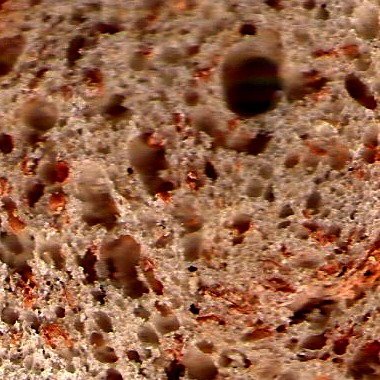
\includegraphics[scale=1.8]{images/salvado19}}}$
$\vcenter{\hbox{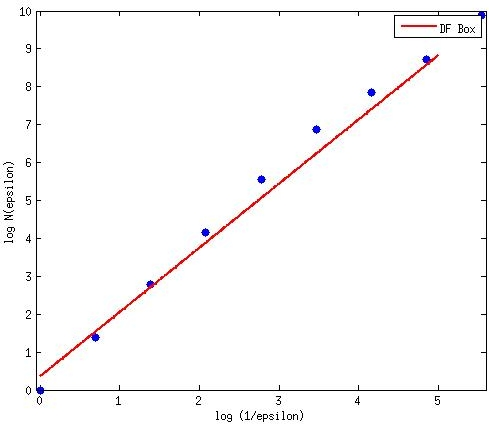
\includegraphics[scale = 0.4]{images/fitbox}}}$
\caption{An image and its computed box dimension}
\label{fig:fitbox}
\end{figure*}

\subsection{The theory behind Multifractal Analysis}
\label{sec:4}

In \cite{Gonzales2008}, several procedures were applied to analyze the bread crumb structure. In that paper, it was shown that a vector of FDs could better characterize those structures. Based on that assumption, in this work multifractal analysis of the bread crumb is carried out. The idea behind multifractal analysis is to examine, in the limit, the local behavior of a measure $\mu$ at each point of the set under study, this means, to find the H\"older exponent $\alpha$ in that point (see below). The {\em multifractal spectrum} $f(\alpha)$ (MFS) is obtained applying this procedure to the entire set, in this case, an image.

Let $E$ be an structure divided in disjoint substructures $E_{i}$ of size $\epsilon$ in such a way that 

\begin{equation}
\displaystyle\bigcup_{i}E_{i} = E.
\end{equation}

Each substructure $E_{i}$ is characterized by a measure $\mu(E_{i})$. From the point of view of multifractal analysis, it is useful to define the H\"older exponent, $\alpha_{i}$, for each substructure $E_{i}$, as a function of $\epsilon$, {\em i.e.}


\begin{equation}
\alpha_{i} \triangleq \frac{ln(\mu(E_{i}))}{ln(\epsilon)},
\label{eqn:eqn4}
\end{equation}
\noindent
and to take the limit when $\epsilon$ tends to $0$. The limit represents the value of the H\"older exponent at a point in the structure, that is

\begin{equation}
\alpha = \lim_{\epsilon\to0}{\alpha_{i}}.
\label{eqn:eqn5}
\end{equation}

The exponent characterizes the local regularity of the structure at a point. To obtain a global characterization of the regularity of the structure it is necessary to obtain the distribution of $\alpha$ in $E$. The range of H\"older exponent values found in the image is partitioned in $M$ sub-ranges (in practice, $M$ is a parameter: the number of FDs). Each $\alpha_{i}$ defines one sub-range. Then a counting $N_{\epsilon}$ of boxes characterized by $\alpha_{i}$ must be done for each of them, related to the value of $\epsilon$, {\em i.e.}

\begin{equation}
f_{\epsilon}(\alpha_{i}) = - \frac{ln(N_{\epsilon}(\alpha_{i}))}{ln(\epsilon)}.
\label{eqn:eqn6}
\end{equation}

When $\epsilon$ tends to $0$, the limiting value is the FD of the structure $E$ characterized by $\alpha$, the Hausdorff dimension (which is calculated by using the Box procedure described) of the $\alpha$ distribution, also known as the {\em multifractal spectrum} $f(\alpha)$ (MFS) \cite{Silvetti2010}, {\em i.e.}

\begin{equation}
f(\alpha) = \lim_{\epsilon\to0}{f_{\epsilon}(\alpha)}.
\label{eqn:eqn7}
\end{equation}

\subsubsection{Practical procedure for the MFS}
There are several techniques described in the literature to obtain the MFS, which lead to different representations of the multifractal information present in the structure. Usually, the method of moments is used \cite{Mendoza2010,Serrano2012}, but it produces a feature vector which is not always suitable for classification tasks. In this work, the implementation presented in \cite{Xu2006} is employed, due to its better classification performance. The implementation first calculates the method of moments and then uses a Legendre transform to obtain the MFS. The procedure consists in partitioning the domain into non-overlapping boxes of length $r$. The $q$-th moment of a measure $\mu$ is defined as
\begin{equation}
M_{r}(q) = \sum{\mu(B(x,r))^{q}},
\label{eqn:eqn8}
\end{equation}
where the sum is over the $r$ mesh squares for which $\mu(B(x,r)) > 0$. To denote the power law behavior of $M_{r}(q)$, $\beta(q)$ is defined as a straight line fit of the values $M_{r}(q)$ with respect to $r$, for $r$ in $1,..,n$. It is shown in \cite{Falconer97}, that the MFS and $\beta(q)$ are related to each other by a Legendre transform as

\begin{equation}
f(\alpha(q)) = q \alpha(q) - \beta(q),
\label{eqn:eqn9}
\end{equation}
where

\begin{equation}
\alpha(q) = \frac{d\beta(q)}{dq}.
\label{eqn:eqn10}
\end{equation}

As previously stated, the $f(\alpha)$ spectrum (MFS) and the generalized dimensions $\beta(q)$ contains the same information, but in this work the first is employed, since it also outperforms the method of moments in classification tasks. Using (\ref{eqn:eqn9}) and (\ref{eqn:eqn10}) the MFS is estimated. As previously said, in this work the implementation in \cite{Xu2006} is used and the parameters of the algorithm are set to default (except for the number of FDs, since they are chosen based on its classification performance).


\subsubsection{Multifractal Measures}
Defining different $\mu$ functions counts for different image features. The first approach is to define $\mu$ in the intensity domain, {\em i.e.}

\begin{equation}
\mu(B(x,r)) = \int_{B(x,r)}{(G_{r} \ast I)} dx,
\label{eqn:eqn11}
\end{equation}
where $\ast$ is the $2D$ convolution operator and $G_{r}$ is a Gaussian smoothing kernel with variance $r$, {\em i.e., } $\mu$ is the weighted average intensity value in the disk of radius $r$ centered at $x$ ($B(x,r)$). This is the density of the intensity function, and it describes how the intensity at a point changes over scale.

The definition of $\mu$ could serve to specific purposes. For instance, if robustness to illumination changes is needed, one choice is to define $\mu(B(x,r))$ on the domain of the energy of the gradients. Let ${ f_{k} , k = 1, 2, 3, 4}$ be four directional differential operators along the vertical, horizontal, diagonal and anti-diagonal directions. Then we define the measurement function $\mu(B(x,r))$ for the image $I$ as in (\ref{eqn:gradient}).

\begin{equation}
\mu(B(x,r)) = (\int_{B(x,r)}{\sum_{k}{(f_{k} \ast (G_{r} \ast I))^{2}} dx)^{1/2}}.
\label{eqn:gradient}
\end{equation}

Another choice is to define $μ(B(x, r))$ as the sum of the Laplacians of the image inside $B(x, r)$ (\ref{eqn:laplacian}).

\begin{equation}
\mu(B(x,r)) = \int_{B(x,r)}|\nabla^2 (G_{r} \ast I)| dx.
\label{eqn:laplacian}
\end{equation}

\subsection{Image Acquisition}
Twenty images of $4$ different commercial bread types ({\em sliced}, {\em baguette}, {\em bran} and {\em sandwich}), counting $80$ images, were obtained in the same day of purchase using an HP PSC 1210 scanner with the following settings: highlight 190, shadows 40, and midtones 1, and they were saved in TIFF format. Images showed a resolution of $380 \times 380$ pixels (the maximum possible area for the four bread types) and $350$ dpi ($1$ pixel $= 0.00527 mm^{2}$). Then the images were converted to gray scale ($8$ bits). In addition, $20$ images of each bread type were acquired with a digital camera, using the same spatial resolution, counting $80$ images. The illumination conditions of these images were different from that of the scanner in order to test for the robustness of the method. We also employed one hundred randomly selected images from the CalTech101~\cite{FeiFei04} dataset in order to test the method's performance with non-bread images. In Fig.~\ref{fig:imagedatabase} three examples of the images used in this paper are shown. In the figure, $2$ images of the {\em baguette} bread type, digitalized using a scanner (left) and a digital camera (center) are shown with a random non bread image from the Caltech101 dataset (right).

\begin{figure*}[htb]
\centering
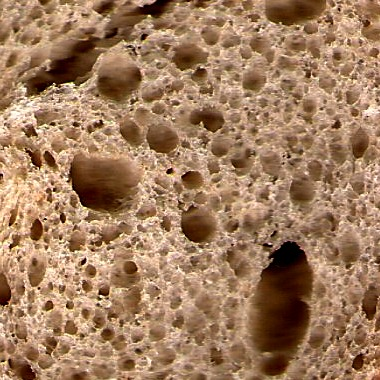
\includegraphics[scale=1.37]{images/baguette20}
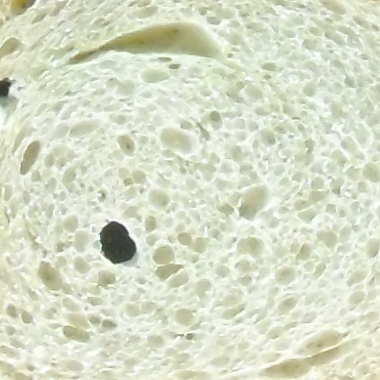
\includegraphics[scale=1.36]{images/b16}
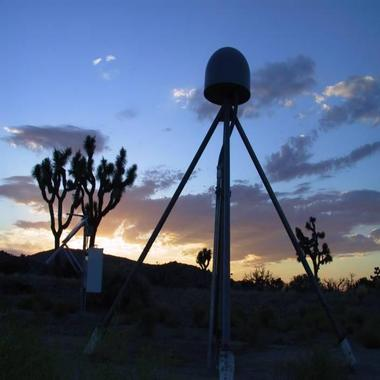
\includegraphics[scale=0.28]{images/image_0300}
\caption{Digitalized images of {\em baguette} bread type and an image of the CalTech101 dataset}
\label{fig:imagedatabase}
\end{figure*}

\section{RESULTS AND DISCUSSION}

\subsection{Data Analysis}
The MFS, using $20$ FDs, was applied for each of the $200$ images ({\em i.e.,} $40$ images of each bread type, and $40$ randomly selected nonbread images, getting $5$ balanced classes).

Self-organizing maps (SOM)~\cite{Kohonen2001} of the vectorized images are useful to visualize these different representation of bread images into a lower dimensional view, in order to understand them better. A SOM map high dimensional data into a (typically) two-dimensional representation, using neighborhood information. Topological information of the original data is preserved.  

Unsupervised SOM of the multifractal representation of bread and non-bread images are shown in Fig.~\ref{fig:somfractal} in a grid of $10\times10$ cells. In the left image, the $5$ classes ({\em e.g.}: {\em baguette}, {\em sliced}, {\em bran}, {\em sandwich} and {\em nonbread}) are shown, while in the right image, the {\em nonbread} class has been removed, and then the SOM was recomputed for the remaining four classes, in order to highlight details among the MFS of the different bread types. The multifractal features SOM appears to show easily separable classes. It seems that a classifier could potentially obtain low classification errors using the multifractal features.
\begin{figure*}
\begin{centering}
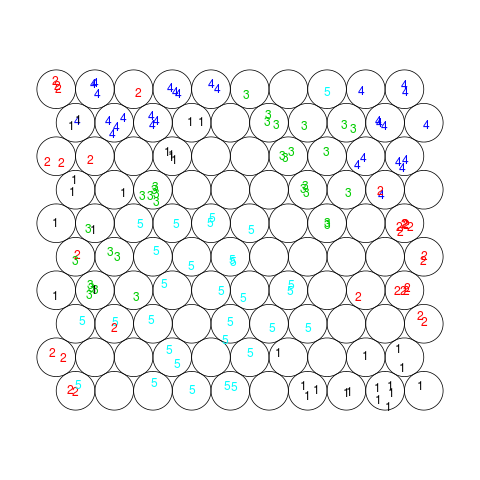
\includegraphics[width=0.45\textwidth]{images/sommultifractal}
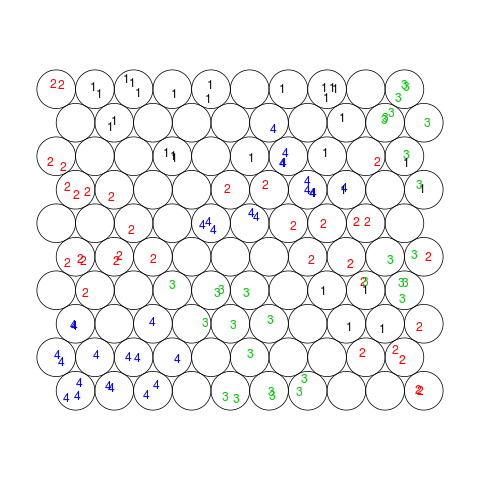
\includegraphics[width=0.45\textwidth]{images/sombreadmultifractal}
\caption{SOM of the bread and non-bread vectorized images (left) and SOM of the vectorized bread images only (right). $1$: {\em baguette}, $2$: {\em sliced}, $3$: {\em bran}, $4$: {\em sandwich}, $5$: {\em nonbread} }
\label{fig:somfractal}
\end{centering}
\end{figure*}

\subsection{Bread Classification}
\label{sec:10}
As previously stated, five classes are defined, {\em e.g.}, {\em baguette}, {\em sliced}, {\em bran}, {\em sandwich} and {\em non-bread}, assigning $40$ images to each class. A comparison is made between the MFS and state-of-the-art features in the computer vision literature. This classification schema corresponds to an intra-class problem, which is harder to solve than an ordinary inter-class one. 

K-fold cross validation is applied to the entire set (with $K=4$), employing three different classifiers: Support Vector Machines (SVM), Random Forests (RF), and Nearest Neighbors (NN). Results show that the MFS presents good classification performance regardless of the classifier employed. The \textsf{libsvm} implementation \cite{Chang2011} was used for the SVM classifier (with RBF kernel). In the case of the RF ($100$ trees) and the NN ($1$ neighbor) classifiers, the \textsf{scikit-learn} python library was employed.

In Table \ref{tab:number}, the classification performance of the method is tested using different numbers of FDs. When $20$ FDs are used, an useful combination of performance and low dimensionality is achieved, so this number of FDs is used in the following calculations.

In Table \ref{tab:mfs}, several combinations of different MFS obtained from the images, and their classification performance are shown. The MFS used in the study were the density of the intensity (MFS in the table), the Laplacian of the intensity (L), and the gradient of the intensity (G). In addition, another test is made, using the CIELab color space. The key advantage of this color space is that it tends to reduce the dependency of the resulting image color on the device used in the capture. The intensity of the images is transformed to the CIELab space, and the MFS of the three separated channels ({\em L}, {\em a}, and {\em b}) are combined together, obtaining a vector of $60$ FDs. This combination showed the best classification performance. It means that adding color information in the $a$ and $b$ channels is useful for better classification of different types of bread crumbs, when different capturing devices are used (in this case, a scanner and a digital camera).

In Table \ref{tab:other}, state-of-the-art features (Haralick, Local Binary Pattern and SIFT features) are computed for the images. The Haralick and Local Binary Pattern features are computed using the {\em mahotas} python library\footnote{https://pypi.python.org/pypi/mahotas}. The best classification performance is obtained using the SIFT features, but a $128$ feature length vector is obtained per image, and, in addition, computational space and time is needed to build internal structures ({\em e.g.} a {\em codebook}). The classification performance of the MFS for the bread crumb database is the highest among the algorithms studied. The MFS captures robust and useful information for classification in low dimensional features. These results also agree with results obtained in \cite{Bosch2011} for the classification of other food products.

\begin{table}[h]
\begin{center}
% table caption is above the table
\caption{classification results with different number of FDs for the MFS}
\vspace{2mm}
\label{tab:number}       % Give a unique label
% For LaTeX tables use
\begin{tabular}{|c|c|c|c|c|}
\hline
SVM & \textbf{96\%} & 94.5\% & 95.5\% \\
\hline
RF  & 91.5\% & \textbf{93.5\%} & 93\% \\
\hline
NN & 88.5\% & \textbf{90.5\%} & 90\% \\
\hline
\hline
\#FDs & 10  & 20 & 30 \\
\hline
\end{tabular}
\end{center}
\end{table}


\begin{table}[h]
\begin{center}
% table caption is above the table
\caption{classification results using different combinations of the MFS}
\vspace{2mm}
\label{tab:mfs}       % Give a unique label
% For LaTeX tables use
\begin{tabular}{|c|c|c|c|c|}
\hline
Method & MFS & MFS+L & MFS+G & CIELab  \\
\hline
\hline
SVM & 94.5\% & 95.5\% & \textbf{97.5\%} & \textbf{97.5\%} \\
\hline
RF  & 93.5\% & \textbf{96\%} & 95\% & \textbf{96\%} \\
\hline
NN & 90.5\% & 90\% & 87\% & \textbf{92\%} \\
\hline
\hline
\#FDs & 20 & 40 & 40 & 60 \\
\hline
\end{tabular}
\end{center}
\end{table}


\begin{table}[h]
\begin{center}
% table caption is above the table
\caption{classification results for different features}
\vspace{2mm}
\label{tab:other}       % Give a unique label
% For LaTeX tables use
\begin{tabular}{|c|c|c|c|c|c|}
\hline
Method & Haralick & Lbp & SIFT\\ % & Zernicke
\hline
\hline
SVM & 94\% & 78.5\% & \textbf{96.5\%} \\ % & 55 
\hline
RF  & 91\% & 71.5\% & \textbf{92\%} \\ % & 58 
\hline
NN & 79\% & 70\% & \textbf{86\%} \\ % & 48.5 
\hline
\hline
\#Features & 13 & 36 & 128 \\
\hline
\end{tabular}
\end{center}
\end{table}


\section{CONCLUSIONS}
The use of multifractal features in bread crumb texture classification showed excellent performance. The MFS demonstrated to be accurate enough to perform a classification of different bread types and also to discriminate non bread from bread images. The classification performance of the MFS for the bread crumb database outperforms other state-of-the-art techniques employed in the computer vision literature. The information present in the MFS of the $L$, $a$ and $b$ channels of the CIElab space color obtained the best classification performance in all the developed tests. This result appears to be a consequence of the different capturing devices used in this work.

The results found could also be applied to validate synthetic samples, in the sense that they should have similar features to the bread type they are trying to simulate. The features found with the MFS could be applied to tune bread crumb quality parameters.

%\section{DESARROLLO}

%\subsection{Instrucciones generales}
%Los trabajos deben estar escritos en formato a doble columna, balanceadas en la \'ultima p\'agina, en un cuadro de 165 mm $\times $ 245 mm. El ancho de las columnas debe ser de 80 mm con 5 mm de distancia entre columnas. Los autores deben enviar los manuscritos \'{u}nicamente en versi\'{o}n electr\'{o}nica, en formato PDF. Los trabajos se recibir\'{a}n en su versi\'{o}n final, no se aceptar\'{a}n res\'{u}menes de trabajos.

%\subsubsection{Importante}
%Las p\'{a}ginas no deben numerarse. Verifique que el archivo enviado no est\'{e} protegido.

%\subsection{Tama\~{n}o de fuentes y espaciado}
%Los trabajos deben estar escritos con espaciado simple. El espaciado puede incrementarse solamente en caso de ser necesario por el uso de sub\'{\i}ndices o super\'{\i}ndices. El tama\~{n}o de las fuentes usadas en el texto de las ilustraciones debe ser, como m\'{\i}nimo, de 2 mm.
%El tama\~{n}o de fuentes para el cuerpo del texto debe ser de 10 puntos (1 punto = 0.35 mm).

%\subsection{Ilustraciones}
%Todas las ilustraciones deben ser originales. Deben ubicarse a lo largo de todo el trabajo, y no agrupadas al final. Los ep\'{i}grafes de las figuras deben ubicarse debajo de las mismas, como se muestra en la Fig. \ref{clementeypereyra}.

%\begin{figure}[ht]
%  \centering{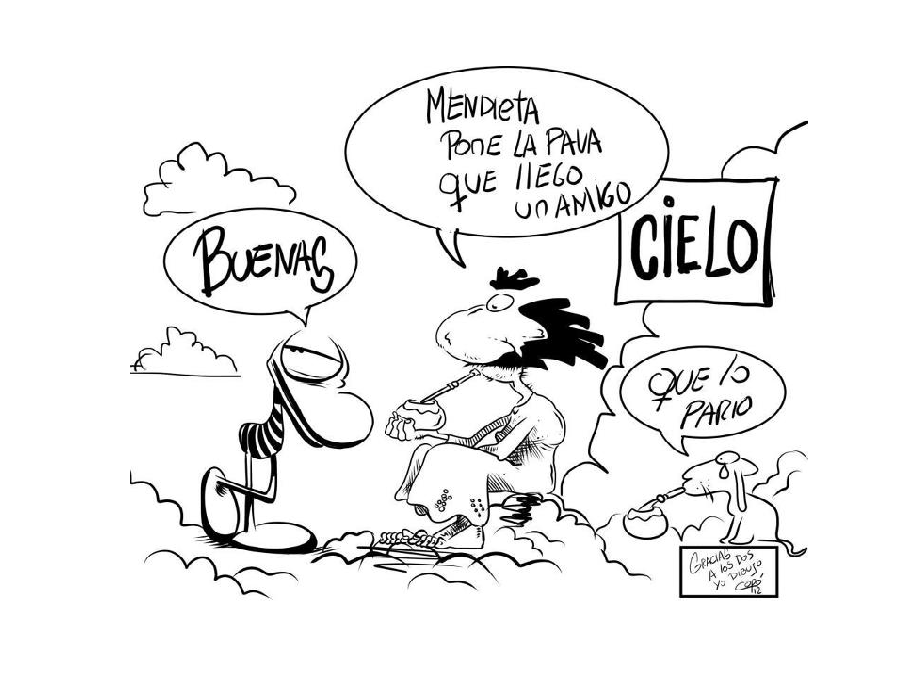
\epsfig{file=clementeypereyra.eps, width=0.8\columnwidth}}
%  \caption{Clemente e Inodoro Pereyra, homenaje a sus creadores.}\label{clementeypereyra}
%\end{figure}

%Los t\'{\i}tulos de las Tablas deben ser breves, y deben ubicarse sobre la tabla correspondiente, como se muestra en la Tabla \ref{posiciones}. Utilice los ambientes tabla y tabla* provistos en rpictyle.sty, si el idioma es el espa\~nol.

%\begin{tabla}[b]
%  \caption{Posiciones Primera B Nacional 2011/12.}\label{posiciones}
%  \vspace{2mm}
%  \centering
%  \begin{tabular}{|c|l|c|} \hline
%  Pos. & Equipo & Puntos\\ \hline\hline
%  $1°$ & River Plate & 73 \\ \hline
%  $2°$ & Quilmes & 72\\ \hline
%  $3°$ & Instituto & 70\\ \hline
%  $4°$ & Rosario Central & 69\\ \hline
%  $\vdots$ & $\vdots$ & $\vdots$ \\ \hline
%  $20°$ & Chacarita Juniors & 32\\ \hline
%  \end{tabular}
%\end{tabla}

%Las ecuaciones, las figuras y las tablas deben numerarse con numeraci\'{o}n ar\'{a}biga.

%El n\'{u}mero de las ecuaciones debe estar alineado junto al margen derecho

%\begin{equation}
%\dot{x}=f_{1}\left( x_{1},t\right) +\alpha x_{2}\sin \left( \theta \right),
%\label{eq1}
%\end{equation}
%mientras que la ecuaci\'{o}n debe ubicarse centrada con respecto a la columna.

%Las palabras ``Figura'' y ``Ecuaci\'{o}n'' deben abreviarse, usando ``Fig.'' y ``Ec.'' cuando se usen en medio de una oraci\'{o}n. Sin embargo, deben
%escribirse en forma completa cuando se empleen al comienzo de la oraci\'{o}n. Cuando se haga referencia a una ecuaci\'{o}n el n\'{u}mero de la misma debe estar entre par\'{e}ntesis y se recomienda evitar utilizar Ec. en los casos en que sea posible. Por ejemplo: ``...de (\ref{eq1}) resulta...''.

%\subsection{Formato de las Referencias}
%En el cuerpo del trabajo, las referencias deben citarse por n\'{u}meros entre corchetes. En el siguiente p\'{a}rrafo se presenta un ejemplo.

%En Rosario dicen, para contrarrestar tanto aburrimiento, que tienen las minas m\'{a}s lindas del pa\'{i}s: parece un invento de la misma \'{i}ndole que la fama que los petisos y los pelados se hicieron de s\'{i} mismos, para compensar por abajo lo que la naturaleza les priv\'{o} de arriba. Yo supongo que esta fama, entonces, es un invento de las rosarinas, para reparar el abandono que padecen los domingos cuando todos los rosarinos, sea por Central o por \~{N}uls, todos se van al f\'{u}tbol \cite{Caloi_2006}. Fontanarrosa adhiere totalmente a este culto. Muestras de esto son muchas de sus obras \cite{Negro_2000,Negro2_2000} o aquellos memorables chistes futboleros como ``Es tan pobre la situaci\'{o}n actual del f\'{u}tbol argentino, que el pr\'{o}ximo cuadrangular amistoso lo vamos a hacer entre tres equipos'' \cite{Negro_1990}.

%La lista de referencias debe escribirse en orden de aparici\'{o}n, siguiendo el estilo general que se muestra en el ejemplo m\'{a}s abajo, correspondiente al provisto por el estilo IEEEtran.bst.

%\section{CONCLUSIONES}
%Es importante que los autores sigan estas ``reglas'' para que los anales puedan elaborarse r\'{a}pida y eficientemente.

% La seccion REFERENCIAS puede realizarse mediante BibTeX, usando
\bibliographystyle{IEEEtran}
\bibliography{bibliografia/bibliografia}

% IEEEtran.bst puede descargarse en: http://www.ctan.org/tex-archive/macros/latex/contrib/IEEEtran/bibtex

% o manualmente

%\begin{thebibliography}{1}

%\bibitem{Caloi_2006}
%C.~Loiseau, ``Homenaje a fontanarrosa,'' in \emph{Proceedings from Senado de la
%  Naci\'{o}n}, Buenos Aires, Argentina, 2006, pp. 165--172.

%\bibitem{Negro_2000}
%R.~Fontanarrosa, \emph{No te vayas, campe\'{o}n}.\hskip 1em plus 0.5em minus
%  0.4em\relax Buenos Aires, Argentina: Editorial {S}udamericana {S}. {A}.,
%  2000.

%\bibitem{Negro2_2000}
%R.~Fontanarrosa, \emph{Puro f\'{u}tbol}.\hskip 1em plus 0.5em minus 0.4em\relax Buenos
%  Aires, Argentina: Ediciones de la {F}lor, 2000.

%\bibitem{Negro_1990}
%R.~Fontanarrosa, ``El f\'{u}tbol es sagrado,'' \emph{Recopilaciones de chistes sueltos},
%  vol. 148, no.~18, pp. 35--48, 1990.

%\bibitem{ej_1}
%A.B.~Autor1, {\em T\'{i}tulo del libro}. Lugar de edici\'{o}n: Editorial, a\~{n}o.

%\bibitem{ej_2}
%A.B.~Autor1, C.D.~Autor2 y E.~Autor3, ``T\'{i}tulo del art\'{i}culo,'' {\em T\'{i}tulo de la revista en cursiva}, volumen, n\'{u}mero, p\'{a}ginas, a\~{n}o.

%\bibitem{ej_3}
%A.B.~Autor1 y C.D.~Autor2, ``T\'{i}tulo del art\'{i}culo,'' {\em T\'{i}tulo del congreso en cursiva}, Lugar, a\~{n}o, p\'{a}ginas.

%\end{thebibliography}

\end{document} 
